%!\mathbf{T}EX root = ../../csuthesis_main.tex
\chapter{考虑边缘计算的无人机航迹规划及任务调度问题}

\section{问题描述及场景设置} \label{sec:description}

\subsection{问题描述}

在交通及交通相关领域中,因为无人机具备隐蔽性好、机动性强、灵活性强,部署容易和应用范围广等特点,可以通过无人机的使用来一定程度上代替人工来完成所需的侦察任务,例如在铁路系统中对铁轨健康状况的检查、事故现场的侦察勘探、高速公路上的交通巡逻任务(见图~\ref{fig:无人机在高速公路上执行交通巡逻任务})等,因此,基于无人机的交通侦察应用逐渐具备了可行性与实用性。

\begin{figure}[!htbp]
    \centering
    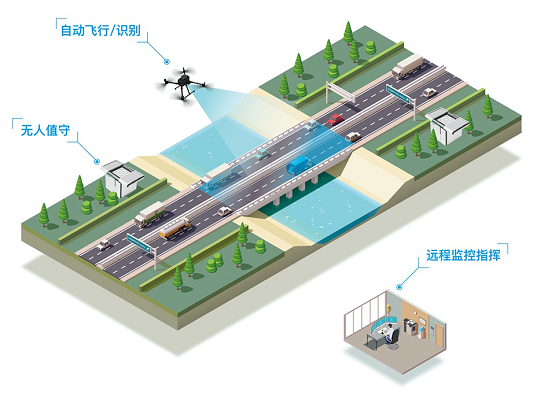
\includegraphics[width=0.7\textwidth]{images/无人机交通侦察应用场景.png}
    \caption{无人机在高速公路上执行交通巡逻任务}
    \label{fig:无人机在高速公路上执行交通巡逻任务}
\end{figure}

本文所研究的问题内容为考虑边缘计算的无人机航迹规划及任务调度问题,为方便讨论,本文将无人机需要执行的侦察任务分为两个部分(见图~\ref{fig:无人机侦察任务组成结构}),分别为收集型任务和计算型任务,其关系如图~\ref{fig:无人机侦察任务关系}所示。收集型任务主要与无人机的摄像设备以及储存设备有关,因此必须由无人机来完成,且该种任务的完成时间是可知的;而计算型任务则需要用到大量算力,若全靠无人机进行计算,则会使得无人机的续航大幅下降,从而使得无人机交通侦察系统效率大幅降低,而全由服务器进行计算,则容易因数据大量同时传输而造成网络拥堵等现象,同样降低了无人机交通侦察系统的效率。

\begin{figure}[!htbp]
    \centering
    \begin{subfigure}[t]{0.4\textwidth}
        \captionsetup{justification=centering}
        \begin{minipage}[b]{\linewidth}
            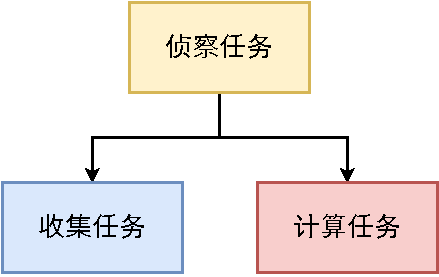
\includegraphics[width=\textwidth]{images/无人机侦察任务组成.pdf}
            \caption{无人机侦察任务组成结构}
            \label{fig:无人机侦察任务组成结构}
        \end{minipage}
    \end{subfigure}
    \begin{subfigure}[t]{0.75\textwidth}
        \captionsetup{justification=centering}
        \begin{minipage}[b]{\linewidth}
            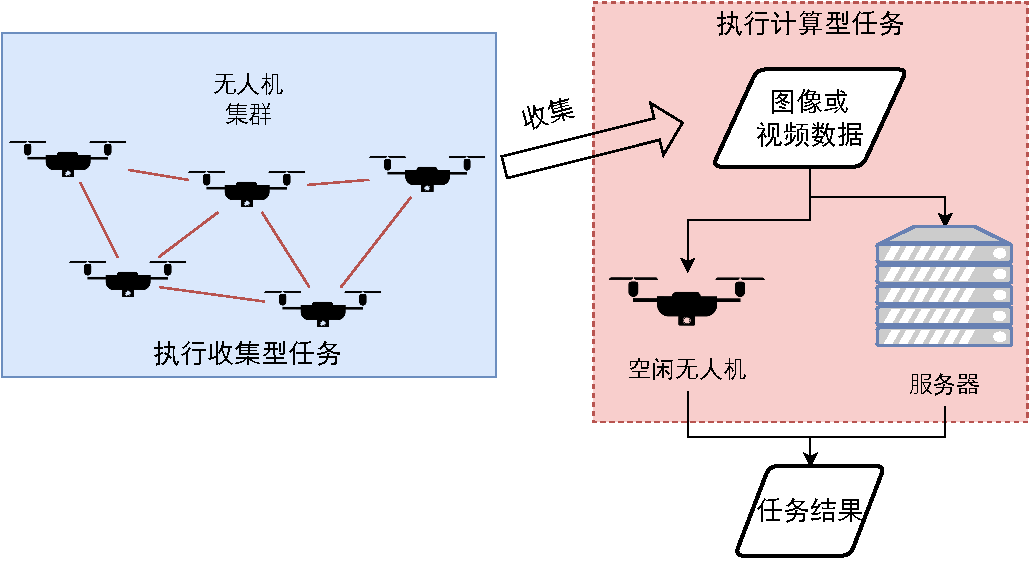
\includegraphics[width=\textwidth]{images/无人机侦察任务关系.pdf}
            \caption{无人机侦察任务关系}
            \label{fig:无人机侦察任务关系}
        \end{minipage}
    \end{subfigure}

    \caption{无人机交通侦察任务组成及关系}
    \label{fig:无人机交通侦察任务组成及关系}
\end{figure}

\begin{figure}[!htbp]
    \centering
    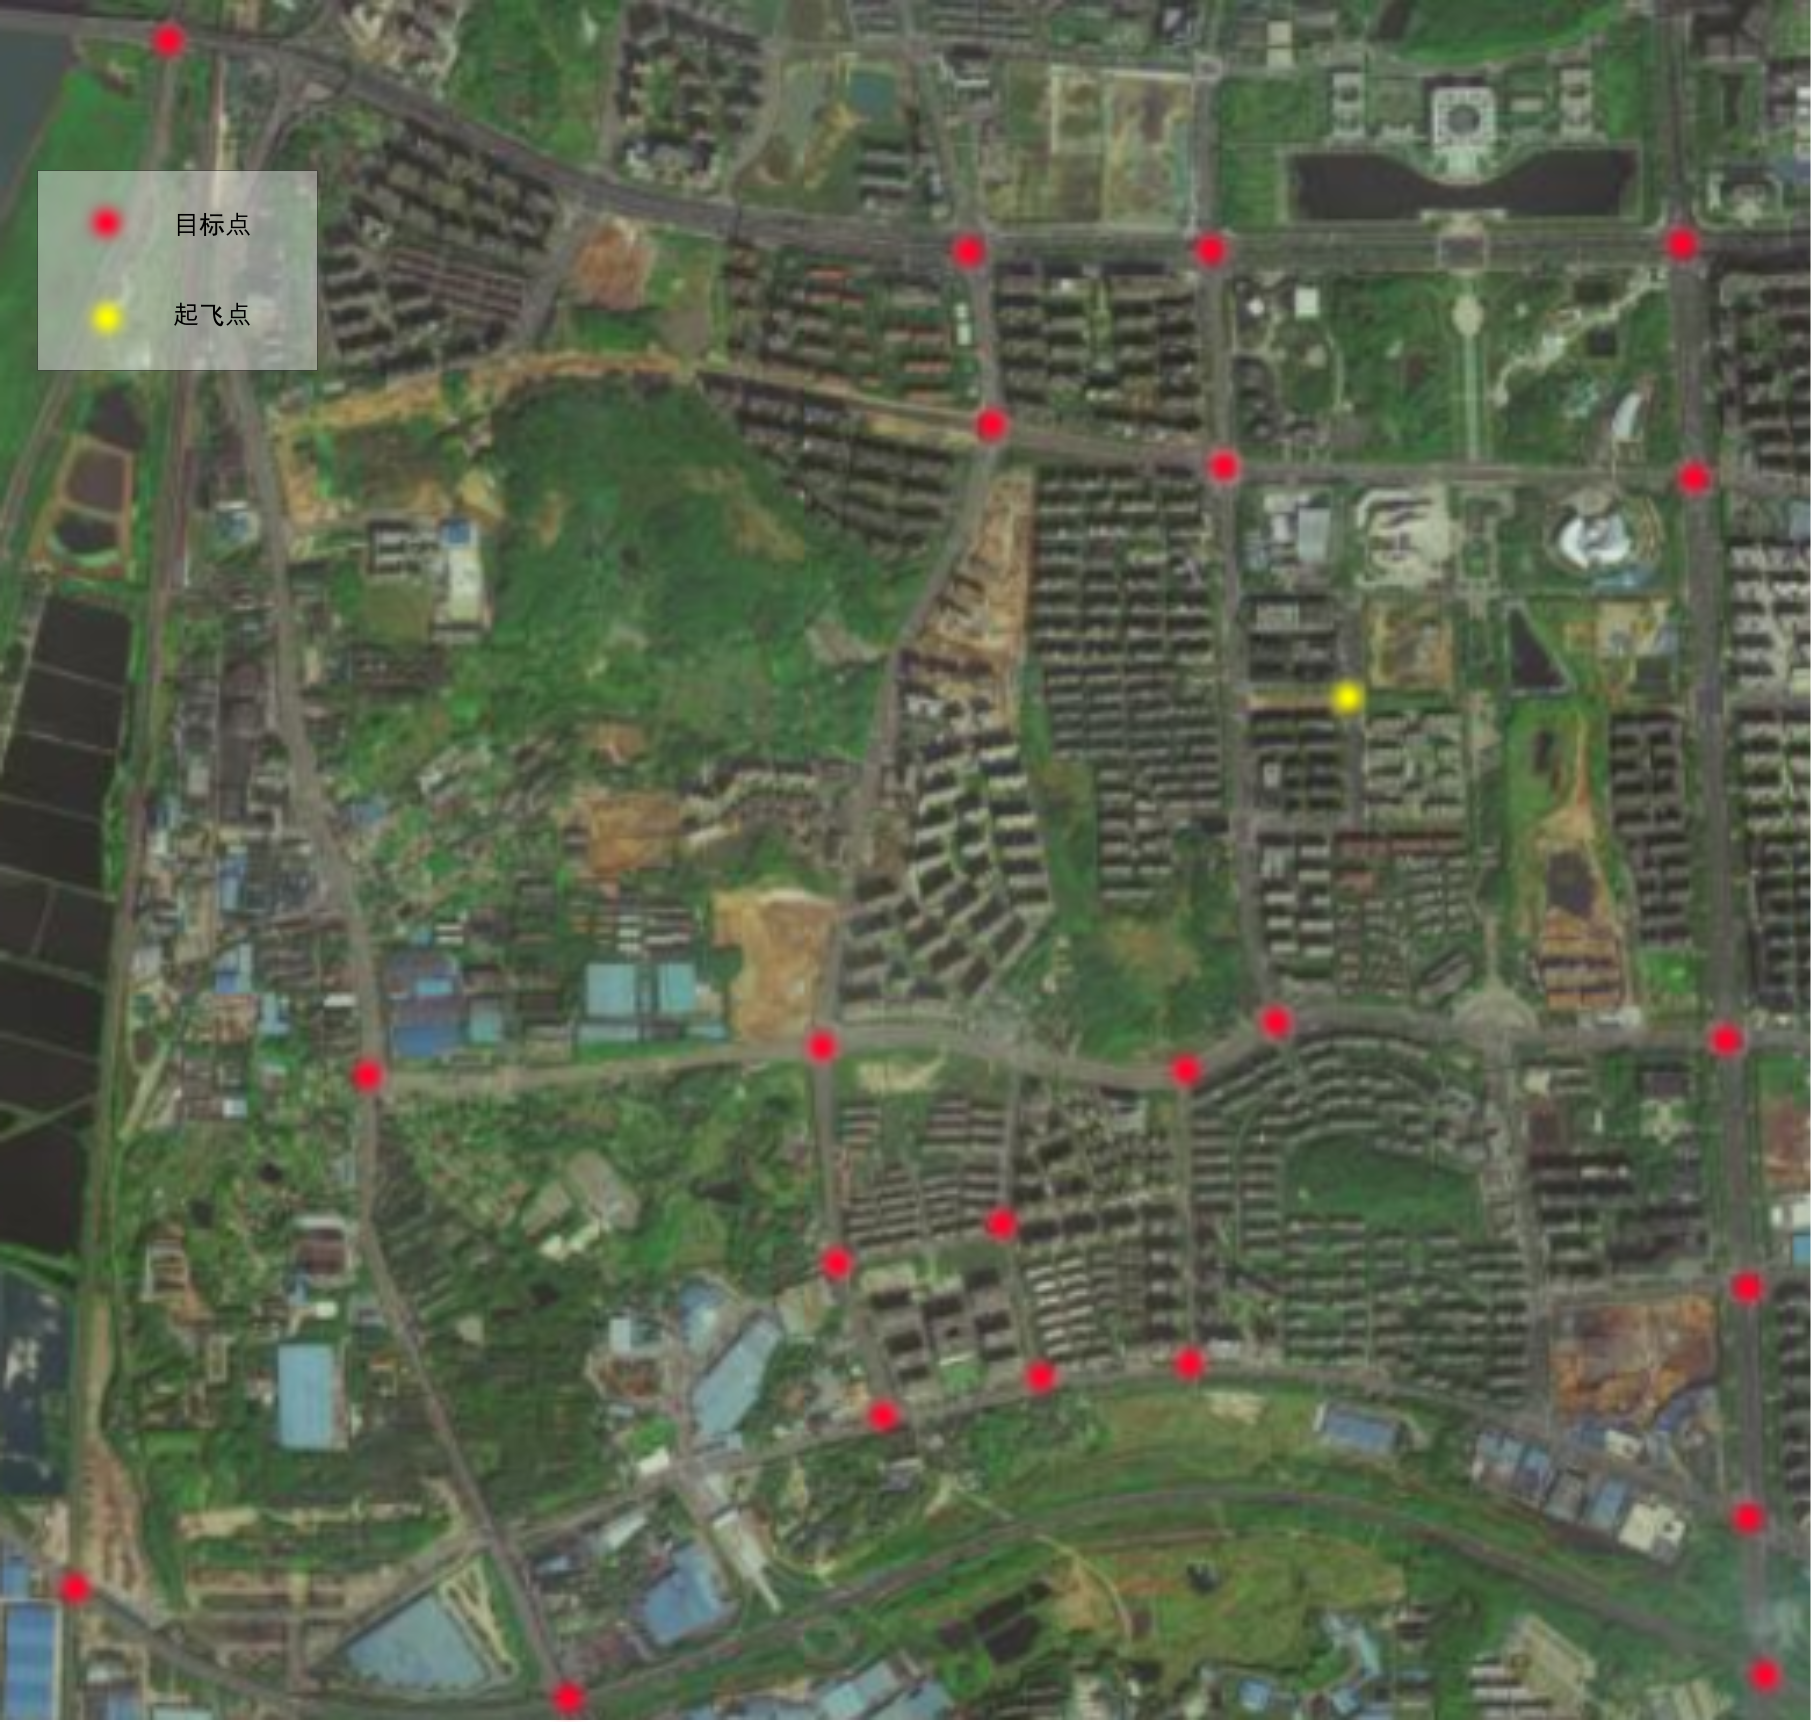
\includegraphics[width=0.7\textwidth]{./images/示例地图}
    \caption{示例地图信息}
    \label{fig:示例地图信息}
\end{figure}

为便于理解上述概念,此处不妨以侦察城市中道路交叉口当前的道路拥堵情况的侦察任务为例,可以将其分解为对该交叉口拍照或录制视频来收集当前道路情况的信息的收集型任务,以及对上述收集到的信息通过神经网络等方法进行计算得出当前该交叉口的道路拥挤情况的计算型任务。对于某个区域而言,存在着22个可能出现拥堵的交叉口(见图\ref{fig:示例地图信息}),需要使用一定数量的无人机来对每个交叉口拥堵情况进行数据收集,在每个任务的数据收集完成后,按照计算资源分配方案将任务数据通过网络通信等方式传输至地面端或边缘端中进行计算,得出各个交叉口拥挤情况后采取相应的措施。

那么基于上述内容,该问题的整体框架如图~\ref{fig:研究问题整体框架}所示,具体流程如下:

\begin{enumerate}[label=(\arabic*)]
    \item {当上级下达指令后,位于地面端的服务器根据任务信息以及地图信息,得到无人机的任务分配方案,包含所需无人机的数量、各无人机所要执行的需进行数据的采集与收集的收集型侦察任务以及相应的飞行航迹;}

    \item {同时服务器根据任务信息、服务器的计算资源以及无人机的计算资源,得到考虑边缘计算下的计算资源分配方案,来安排执行各计算型任务的设备;}

    \item {之后根据得到的无人机的收集型任务分配方案,将对应指令传输至无人机集群中,无人机根据接受到的指令进行飞行控制;}

    \item {在无人机按照飞行航迹进行飞行时,若飞行航迹中存在与航迹冲突的障碍物,那么需要实时对航迹进行修订,使得无人机能够在与障碍物发生碰撞之前对障碍物进行回避;}

    \item {在无人机到达目标点并采集完任务数据后,按照计算资源分配方案将任务数据通过网络通信等方式传输至地面端或边缘端中进行计算;}

    \item {最后根据计算所得的侦察任务结果采取对应的措施。}
\end{enumerate}

\begin{figure}[!htbp]
    \centering
    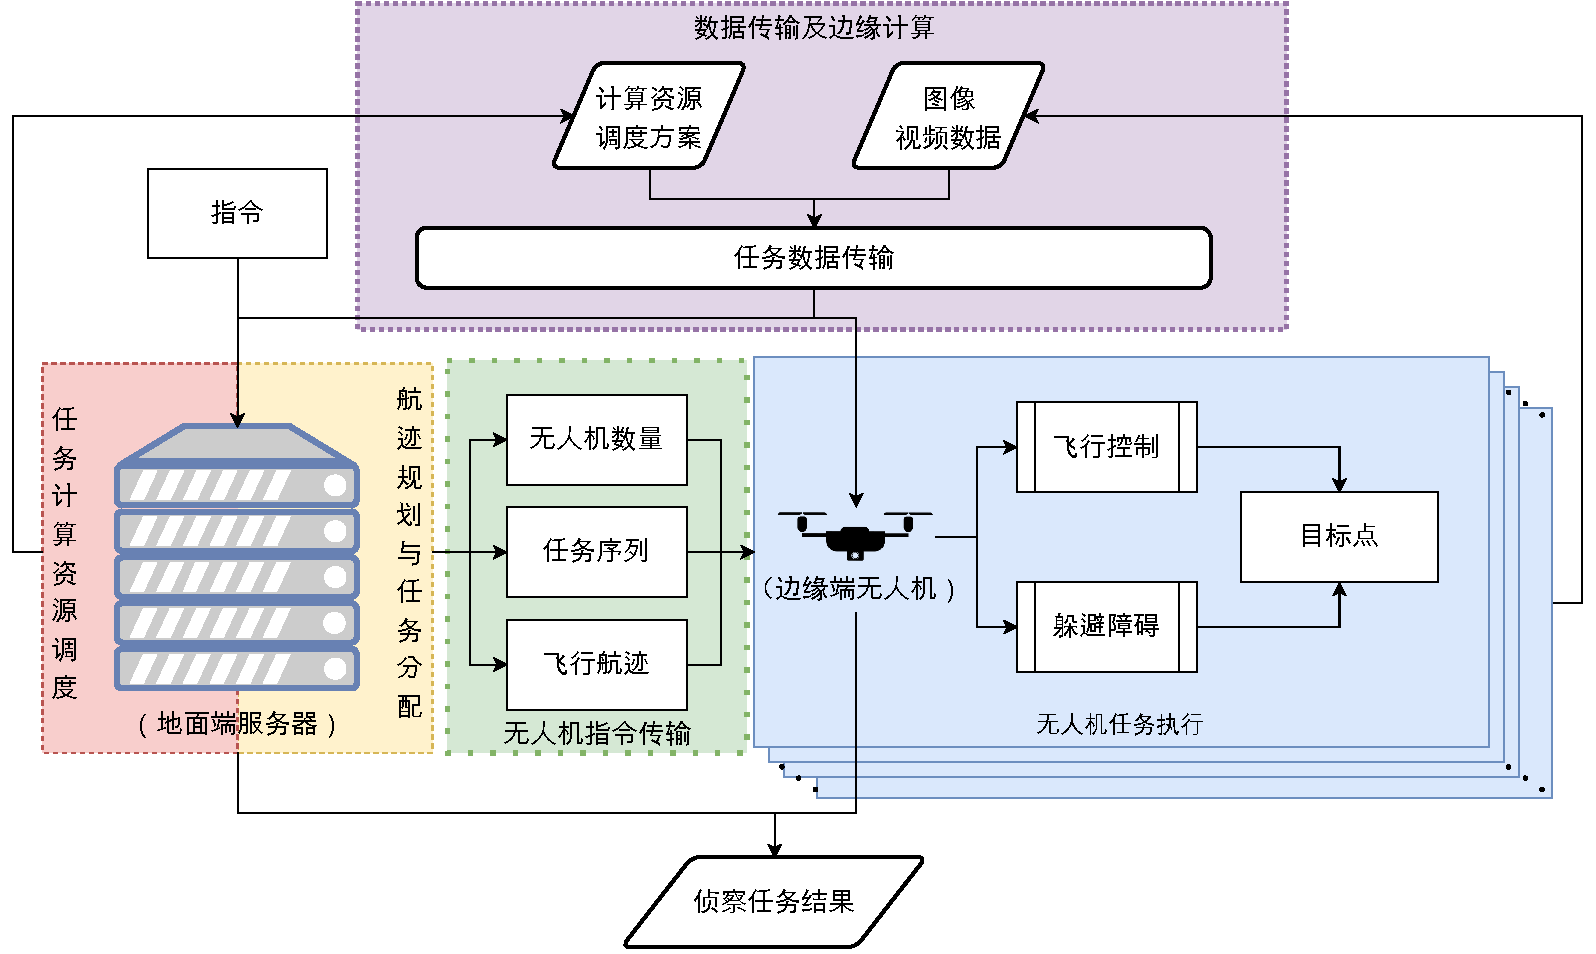
\includegraphics[width=\textwidth]{images/毕设问题框架.pdf}
    \caption{本文研究问题整体框架}
    \label{fig:研究问题整体框架}
\end{figure}

其中数据与指令的传输不在本文的研究范围内,因此本文将考虑边缘计算的无人机航迹规划及任务调度问题分为两个子问题,分别为面向边缘计算的任务计算资源调度优化问题、多无人机的航迹规划及任务分配问题。

\begin{figure}[!htbp]
    \centering
    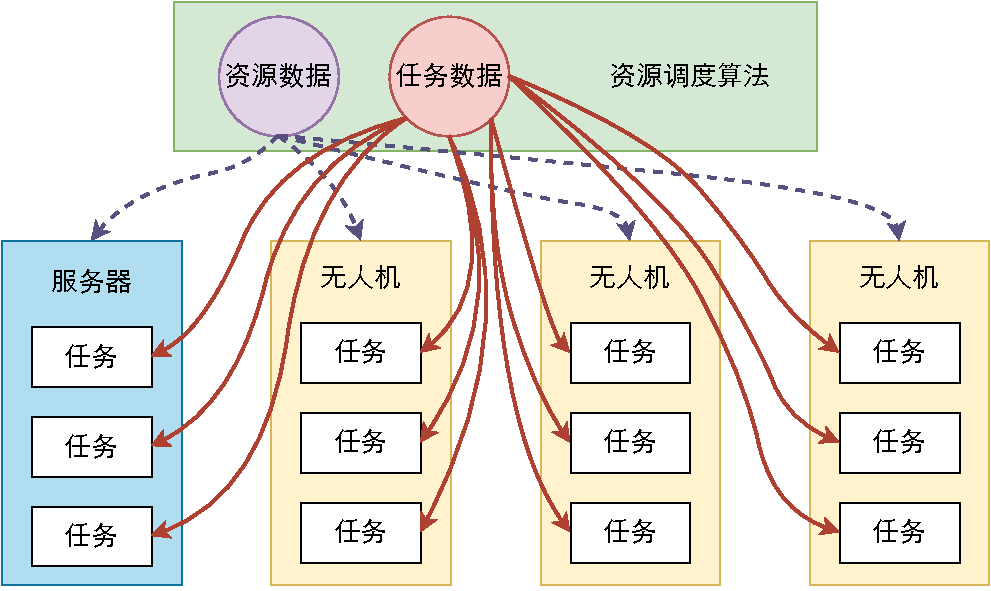
\includegraphics[width=0.7\textwidth]{images/资源调度算法.pdf}
    \caption{资源调度算法示意图}
    \label{fig:资源调度算法示意图}
\end{figure}

\begin{figure}[!htbp]
    \centering
    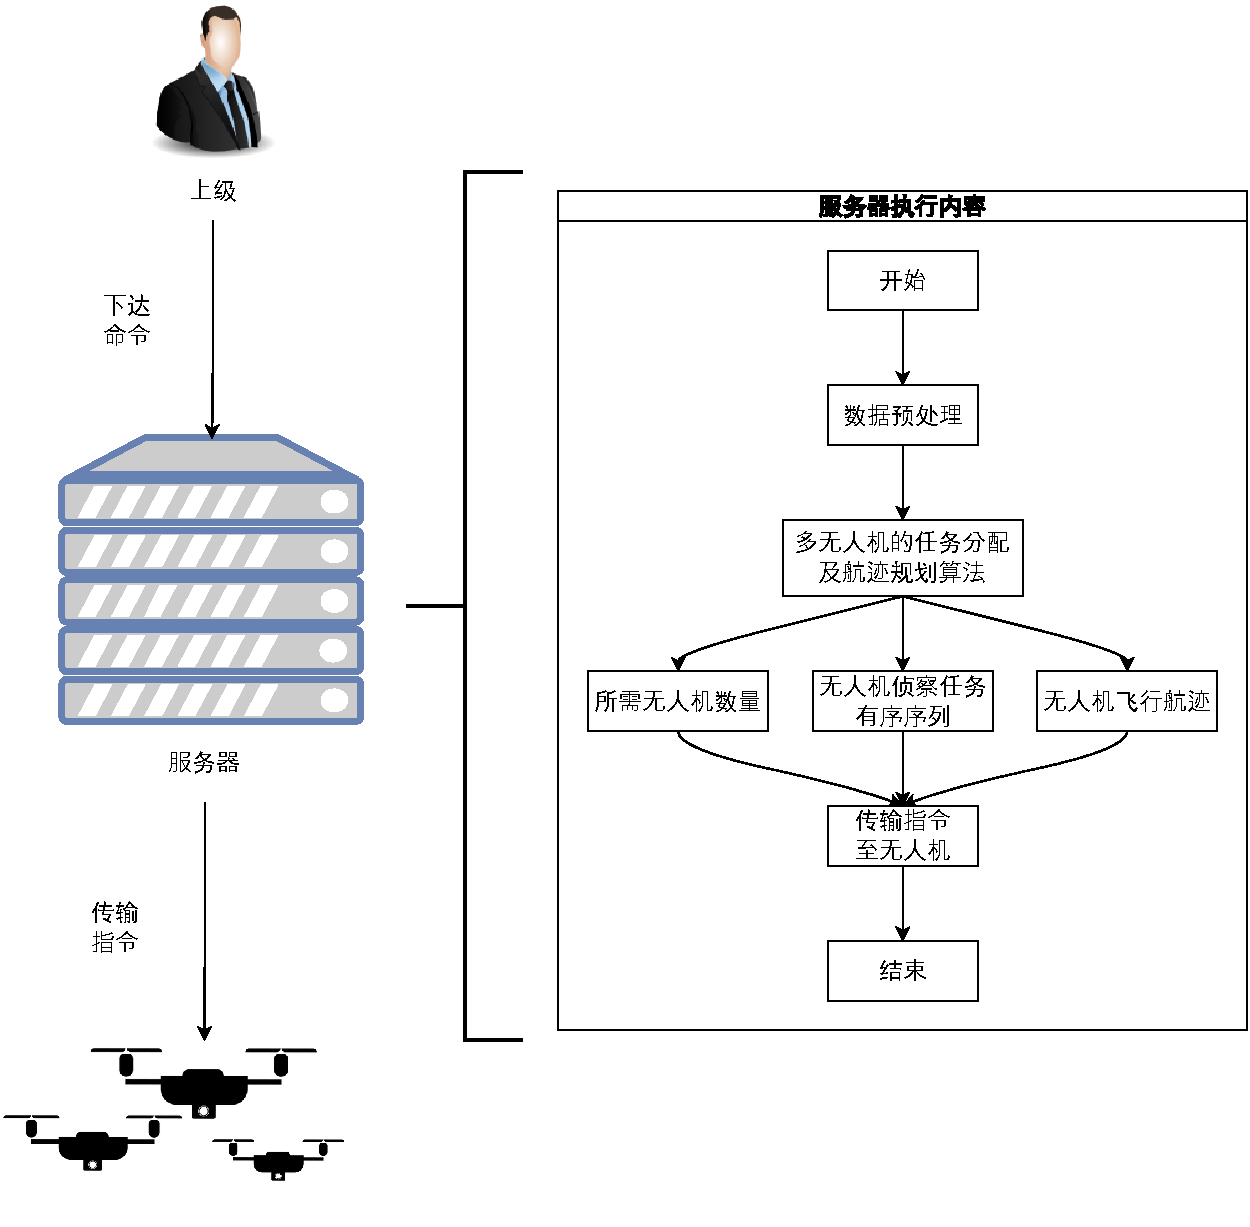
\includegraphics[width=0.9\textwidth]{images/多无人机的任务分配及航迹规划流程.pdf}
    \caption{多无人机的航迹规划及任务分配流程}
    \label{fig:多无人机的航迹规划及任务分配流程}
\end{figure}

任务计算资源的调度优化问题是在有限的计算资源及设备的情况下,通过一定的算法生成任务计算资源调度方案来安排计算设备完成指定的计算型任务,使得整个系统的成本较低,具备实用性的问题。因为无论是无人机集群还是服务器,其计算资源存在着一定的上限,而过多的布置无人机或服务器的数量,虽然能够确保所有计算任务都能够及时准确地完成计算,但会极大增加系统的成本,且有非常严重的资源浪费,而对计算资源进行充分地利用,能极大降低应用成本,提高系统的可行性,因此,在有限计算资源下对任务计算资源进行调度优化十分重要。对于整个系统而言,由于侦察任务有不同的种类,每个种类对于计算资源的要求各有不同,而无人机的计算资源,无论是可用CPU核心数还是可用内存,都与服务器存在着较大的差异,因此会存在着对于不同的侦察任务,其在不同设备的计算完成时间不一致的现象。与此同时,由于无人机与无人机、无人机与服务器之间是通过无线通信技术进行交流,因此还会存在着诸如通信延迟、传输丢包等通信问题,如何处理这些问题也是解决任务计算资源的调度优化问题中极为重要的内容。本文则提出一种具备负载均衡的面向边缘计算的任务计算资源分配算法(如图~\ref{fig:资源调度算法示意图}中的资源调度算法),根据设备的计算资源情况以及任务的需求情况,将不同的任务分配至无人机与服务器计算,合理有效地对计算资源进行分配。

由于无人机的计算功率,即是否进行对侦察任务数据的计算、计算所耗费的时间等,都会影响到无人机飞行的续航时间,而这不利于本章算法所涉及的资源分配问题的解决,同时也会对另外两个问题产生影响。因此,本章假定无人机的续航时间为可容许的最小续航时间,而剩余的续航时间所对应的计算资源则供给给可能需要进行计算的计算型侦察任务的数据。

如图~\ref{fig:多无人机的航迹规划及任务分配流程}所示,多无人机的航迹规划及任务分配问题是在给定收集型任务信息、地图信息后,由服务器根据所给信息,在尽可能短的时间内使用一定的算法确定完成任务所需的无人机数量、各无人机所执行的最优侦察任务有序序列、各无人机执行任务序列的最优飞行航迹,以便控制无人机完成所给的侦察任务的问题。

\subsection{场景设置}

本文以无人机群在城市环境中低空飞行,完成指定区域的目标识别任务、目标搜索任务等侦察任务为研究的应用场景。为简化整体问题便于研究,本文设定执行侦察任务所用无人机为同一型号的旋翼无人机,环境为存在障碍物高低差且障碍物数量较多、较为复杂的城市环境作为测试场景。

\section{模型假设}

为了能够集中力量研究主要问题,确定研究问题的边界,便于开展问题的研究,在不影响模型建立和求解算法的基础上,本文对考虑边缘计算的无人机航迹规划及任务调度问题提出下列合理的假设以简化模型:

\begin{enumerate}
    \item {无人机应用场景中,所有的障碍物均以长方体进行拟合;}

    \item {服务器具有的计算能力和计算资源均强于无人机,使得在计算同一侦察任务的数据使服务器能够以更快的速度完成任务以及同时能够完成更多任务;}

    \item {通信传输的延迟不会受到除了设备间的欧式距离以外的因素的影响;}

    \item {无人机与无人机、无人机与服务器之间的网络延迟具备可预测性,即能够根据无人机位置、通信时间等预测设备间的网络延迟;}

    \item {无人机携带的传感器能够实时感知所在环境的障碍物信息,能够获取无人机与障碍物的距离等所需信息;}

    \item {无人机能够自行处理部分侦察任务的数据,但计算时间会长于服务器计算时间;}

    \item {服务器拥有的地图数据为最新数据,与现实地图不存在较大的差距变化,例如现实中存在的大楼在地图数据中显示为空地,仅存在微小的变化,例如大楼外部的空调外机;}

    \item {无人机进行转向活动时耗费的时间不计;}

    \item {同一任务在相同设备上运行时间具备可预测性,即能够根据任务类型、任务所需内存及设备类型预测该任务在该设备下完成计算所需时间;}

    \item {无人机和服务器都可以同时执行任意数量的任务且不会影响它们的运算速度。}
\end{enumerate}

\section{符号定义}

表~\ref{tab:数学符号及意义}为小节~\ref{sec:math_model}中的数学模型所使用的数学符号:

\begin{longtable}{c C{0.8\textwidth}}
    \caption{数学符号及意义} 
    \label{tab:数学符号及意义} \\
    \hline
        \textbf{符号} & \textbf{意义}\\
    \hline
        \( N \) & 无人机数量 \\
        \( \mathbf{O} \) & 障碍物集合 \\
        \( \ell_\text{max} \) & 无人机最大航程 \\
        \( C_k \) & 第\( k \)台无人机的航迹坐标 \\
        \( d(C_k) \) & 根据第\( k \)台无人机的航迹坐标计算得出的飞行航程 \\
        \( \mathbf{J} \) & 任务集合 \\
        \( J \) & 任务数量 \\
        \( i \) & 第\( i \)个任务 \\
        \( \mathbf{T} \) & 任务类型集合 \\
        \( \mathbf{T}_i \) & 第\( i \)个任务的类型 \\
        \( k \) &  第\( k \)台设备 \\
        \( \mathbf{M} \) & 设备集合 \\
        \( M \) & 设备数量 \\
        \( G_k \) &  第\( k \)台设备为地面端,0则不是,1则是 \\
        \( L_k \) & 第\( k \)台设备的最大内存 \\
        \( W_i \) & 执行第\( i \)个任务所需内存 \\
        \( D_{i k} \) & 第\( i \)个任务上传至第\( k \)个设备的通信延迟,不需要上传时为\( 0 \) \\
        \( X_{i k} \) & 第\( i \)个任务是否由第\( k \)个设备处理 \\
        \( F_{i k} \) & 第\( i \)个任务上传至第\( k \)个设备的上传速度,不需要上传时为\( \infty \) \\
        \( P(W_i, \mathbf{T}_i, G_k) \) & 根据第\( i \)个任务的所需内存和任务类型预测在第\( k \)个设备中开始处理到处理完成所需的时间的函数 \\
        \( t_{i k} \) & 第\( i \)个任务从开始执行到在第\( k \)个设备中处理到执行完成总共的时间 \\
        \( S_{i} \) & 第\( i \)个任务开始执行的时间 \\
        \( C_{i} \) & 第\( i \)个任务执行完成的时间 \\
        \( C_{\text{max}} \) & 所有任务中最后完成执行的任务的完成时间 \\
    \hline
\end{longtable}

\section{数学模型} \label{sec:math_model}

本小节根据小节~\ref{sec:description}中对无人机交通侦察动态规划问题进行分解后的问题分别建立任务计算资源调度模型(见小节~\ref{sec:resouce_scheduling_model})、多无人机航迹规划及任务分配模型(见小节~\ref{sec:assignment_model})。

\subsection{任务计算资源调度模型} \label{sec:resouce_scheduling_model}

\begin{equation}
    \min F_1 = (C_{\text{max}}, C_{\text{max}} \cdot M - \sum^J_{i} \sum^M_{k} t_{ik} X_{i k})  \label{eq:target1}
\end{equation}

\begin{equation}
    C_{\text{max}} = \max(C_{i}) \label{eq:target_mean1}
\end{equation}

\begin{equation}
    C_{i} = S_{i} + \sum_{k \in [1, M]} t_{ik} X_{ik} \label{eq:completion_time3}
\end{equation}

\begin{equation}
    t_{ik} = 2 D_{ik} + \frac{W_i}{F_{ik}} + P(W_i, \mathbf{T}_i, G_k) \label{eq:compute_time3}
\end{equation}

s.t.

\begin{equation}
    \sum_{i \in [1, J]} W_i X_{ik} < L_k, \forall_{t \in [0, C_{\text{max}}]} \forall_{k \in [1, M]} \label{eq:mem_restrant3}
\end{equation}

\begin{equation}
    \sum_{k \in [1, M]} X_{ik} = 1, \forall_{i \in [1, J]} \label{eq:only_one3}
\end{equation}

\begin{equation}
    X_{ik} = \{0, 1\}, \forall_{i \in [1, J], k \in [1, M]} \label{eq:integer_restrant3}
\end{equation}

\begin{equation}
    \sum_{i \in [1,  J]} \sum_{k \in [1, M]} X_{i k} = J \label{eq:all_mission3}
\end{equation}

\begin{equation}
    P(W_i, \mathbf{T}_i, G_k) > 0, \forall_{i \in [1, J], k \in [1, M]} \label{eq:predict_function3}
\end{equation}

\begin{equation}
    C_{i} > S_{i} \ge 0, \forall_{i \in [1, J], k \in [1, M]} \label{eq:time_restrant3}
\end{equation}

\begin{equation}
    D_{ik}, F_{ik}, L_{i}, W_{i}, t_{ik}, G_{k} > 0, \forall_{i \in [1, J], k \in [1, M]}, G_{k} \in \mathbb{Z} \label{eq:variable_restrant3}
\end{equation}

其中,式~\ref{eq:target1}为模型的目标函数,该目标值的含义如表~\ref{tab:数学符号及意义}中所示,即任务完成时间\( C_{\text{max}} \)最短、设备空闲时间\( C_{\text{max}} \cdot M - \sum^J_{i = 1} \sum^M_{k = 0} t_{ik} X_{i k} \)最少,而设备空闲时间最少是为了确保设备的资源利用率,使得本文所提出的算法具备负载平衡的功能,其中任务完成时间的计算方式如式~\ref{eq:target_mean1}所示;而对于第\( i \)任务的完成时间\( C_{i} \),则由式~\ref{eq:completion_time3}中所示,由任务的开始执行时间\( S_{i} \)与决策确定的完成所需时间\( \sum_{k \in [1, M]} t_{ik} X_{ik} \)之和决定;而对于第\( i \)个任务在第\( k \)台设备上的完成所需时间\( t_{ik} \),则由式~\ref{eq:compute_time3}所决定,其中分别为上传延迟\( D_{i k} \)、上传时间\( \frac{W_i}{F_{i k}} \)、计算时间\( P(W_i, \mathbf{T}_i, G_k) \)和下载延迟\( D_{i k} \)所决定。

在上述基础上,本文对整个场景进行了约束,其中式~\ref{eq:mem_restrant3}确保在任意时刻下,任意设备所执行的任务所需内存总和不超过该设备最大可用内存;式~\ref{eq:only_one3}和~\ref{eq:integer_restrant3}确保每一个任务只会且只能由一台设备所执行;式~\ref{eq:all_mission3}确保每一个任务都会被完成;式~\ref{eq:predict_function3}是确保对任务完成所需时间的预测在一个符合实际的范围;式~\ref{eq:variable_restrant3}则式对各个变量进行约束。

\subsection{多无人机航迹规划及任务分配模型} \label{sec:assignment_model}

\begin{equation}
    \min F_2 = (\sum^N_{k=1} d(C_k), N)  \label{eq:target2}
\end{equation}

s.t.

\begin{equation}
    C_k \notin \mathbf{O}, \forall_{k \in [1, N]} \label{eq:route_constrain}
\end{equation}

\begin{equation}
    d(C_k) \le \ell_\text{max} , \forall_{k \in [1, N]} \label{eq:route_length_constrain}
\end{equation}

\begin{equation}
    C_1 \cap C_2 \cap \ldots \cap C_N = \emptyset \label{eq:crash_constrain}
\end{equation}

其中,式~\ref{eq:target2}表示优化目标为无人机数量最少,且无人机的飞行航程之和最小;式~\ref{eq:route_constrain}为
无人机与障碍物的飞行避撞约束,即无人机在飞行航迹中任意一点均不与障碍物接触,从而避免飞行过程中发生无人机因与障碍物碰撞而损毁的情况;
式~\ref{eq:route_length_constrain}为无人机的航程约束,确保每一无人机飞行航迹的飞行航程均不超过其最大航程,从而
避免无人机因续航耗尽导致的损毁;式~\ref{eq:crash_constrain}无人机与无人机的飞行避撞约束,
即无人机在飞行航迹中任意一点均不与其他无人机接触,从而避免飞行过程中发生无人机因与其他无人机碰撞而损毁的情况。

\section{本章小结}

本章主要对无人机航迹规划及任务调度问题进行具体描述和分析,同时将该问题分解成了两个子问题,分别是任务计算资源的调度优化问题、多无人机的航迹规划及任务分配问题,并在提出合理假设和数学符号的基础上,分别建立任务计算资源的调度优化问题、多无人机的航迹规划及任务分配问题的数学模型,并对各个模型的目标函数及约束条件进行了说明。

\newpage
